\section{Test-circuit results (8-bit parity checker)}
\subsection{Circuit and SPICE reference}
The assigned circuit is an 8-bit parity checker: the output is $1$ when an odd number of the eight inputs is $1$. The netlist is not provided, so it was designed (assumption, Appendix~\ref{app:assumptions}) as a balanced
tree of seven XOR2 cells (four, two and one cell per level), each XOR2 built from four NAND2 gates,
\[ n_1=\overline{ab},\quad n_2=\overline{a\,n_1},\quad n_3=\overline{b\,n_1},\quad y=\overline{n_2\,n_3}, \]
i.e.\ 28 NAND2 gates and 112 transistors, with the NAND2 sizing of Section~\ref{sec:gates_method}. All eight primary inputs are ideal sources at exactly $0$ or $V_{DD}$, and the ground rail contains a $0$\,V current probe as in the gate netlists.

The complete netlist was simulated for all $2^8=256$ input vectors at the same 200 corners as the gates ($51{,}200$ runs), each run at the mandated solver options and cross-checked against the tight solve (Section~4).
All 51{,}200 runs converged with the mandated options, the cross-check agreed everywhere, the output was at the correct logic rail in every run (so the circuit implements the parity function), and no leakage was negative.

\subsection{Hierarchical ML prediction}
For every input vector the logic value at the inputs of each of the 28 gates is obtained by logic propagation; the gate model of Part B for that input combination and that corner gives the gate leakage (its SPICE-recorded node voltages are those of the isolated gate at the same corner), and the 28 gate leakages are summed. This assumes that every gate input sits exactly at $0$ or $V_{DD}$ and ignores loading between gates.

\subsection{Results}
\begin{table}[H]
\centering
{\small
\begin{tabular}{lrrrrr}
\toprule
input vectors & SPICE median [A] & ML median [A] & bias & median err & 95th pct err \\
\midrule
all 51,200 runs & $2.87\times10^{-9}$ & $2.79\times10^{-9}$ & 0.96\% & 6.38\% & 19.12\% \\
0 ones in input & $3.33\times10^{-9}$ & $3.24\times10^{-9}$ & 1.16\% & 5.93\% & 17.15\% \\
1 ones in input & $3.19\times10^{-9}$ & $3.04\times10^{-9}$ & 1.08\% & 6.13\% & 18.01\% \\
2 ones in input & $3.10\times10^{-9}$ & $2.91\times10^{-9}$ & 1.03\% & 6.16\% & 18.90\% \\
3 ones in input & $2.97\times10^{-9}$ & $2.87\times10^{-9}$ & 0.99\% & 6.31\% & 19.02\% \\
4 ones in input & $2.90\times10^{-9}$ & $2.79\times10^{-9}$ & 0.96\% & 6.39\% & 19.12\% \\
5 ones in input & $2.80\times10^{-9}$ & $2.73\times10^{-9}$ & 0.93\% & 6.50\% & 19.24\% \\
6 ones in input & $2.74\times10^{-9}$ & $2.69\times10^{-9}$ & 0.91\% & 6.45\% & 19.35\% \\
7 ones in input & $2.74\times10^{-9}$ & $2.68\times10^{-9}$ & 0.90\% & 6.54\% & 19.26\% \\
8 ones in input & $2.83\times10^{-9}$ & $2.72\times10^{-9}$ & 0.94\% & 6.46\% & 19.12\% \\
\bottomrule
\end{tabular}
}
\caption{Test-circuit results (8-bit parity checker): all runs and split by the number of ones in the input vector (200 corners each).}
\label{tab:circuit}
\end{table}


\begin{table}[H]
\centering
{\small
\begin{tabular}{lrrrr}
\toprule
comparison & bias & median err & 95th pct err & mean accuracy \\
\midrule
ML(circuit) vs SPICE(circuit) & 0.96\% & 6.38\% & 19.12\% & 92.49\% \\
sum of isolated-gate SPICE vs SPICE(circuit) [loading effect only] & 0.00\% & 0.00\% & 0.01\% & 100.00\% \\
\bottomrule
\end{tabular}
}
\caption{Where the circuit-level error comes from: ML versus circuit SPICE, and the sum of the isolated-gate SPICE leakages versus circuit SPICE (loading effect only).}
\label{tab:cdecomp}
\end{table}


\begin{figure}[H]\centering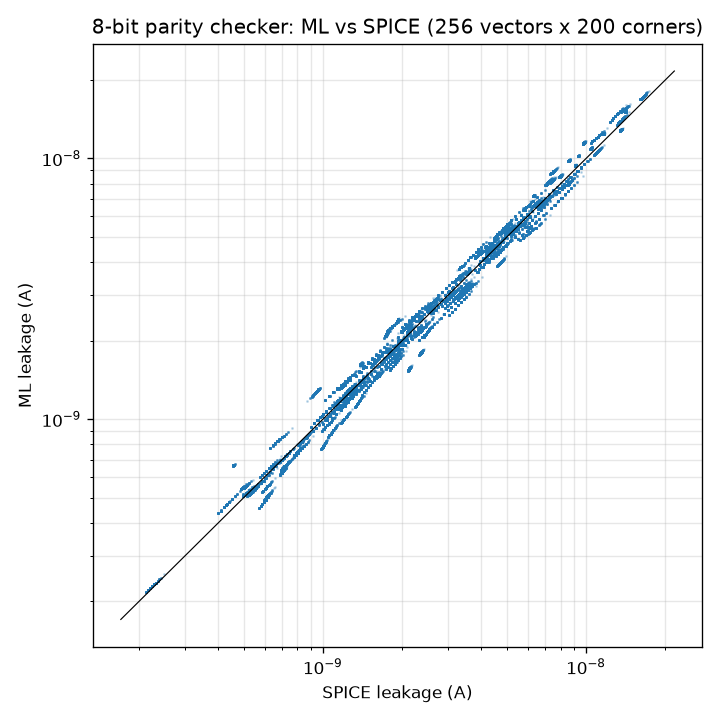
\includegraphics[width=.72\textwidth]{circuit_parity.png}\caption{ML versus SPICE leakage of the parity checker, all 51{,}200 runs (log axes).}\label{fig:cparity}\end{figure}
Over all 51{,}200 runs the median error is 6.4\,\%, the 95th percentile 19.1\,\% and the mean accuracy 92.5\,\%, with a small positive bias ($+1.0$\,\%). The error does not depend on the input vector
(5.9--6.5\,\% median for 0 to 8 ones in the input), and it is close to the gate-level accuracy (median 5.5\,\%), \emph{not} markedly worse as the assignment anticipates.
The reason is visible in the second table: for these rail-to-rail inputs the sum of the SPICE leakages of the isolated gates reproduces the SPICE leakage of the whole circuit to $10^{-4}$, so ignoring the loading between gates costs essentially nothing; the entire error is the ML error of the gate models.

\paragraph{Errors do not average out.} One might expect the errors of the 28 gates to cancel in the sum. They do not, because all gates of the circuit share one corner (same $V_{DD}$, temperature and process draw) and therefore share the same systematic model error: the mean signed error of a corner varies by $9.9$\,\% (standard deviation) between corners but by only $0.2$\,\% between the 256 input vectors at one corner,
and the per-corner circuit error is correlated with the per-corner error of the NAND2 gate (correlation coefficient $0.87$). The circuit error therefore tracks the corner-dependent accuracy of the transistor models (median error 8.3\,\% for $-40$--$0\,^\circ$C, 4.3--4.9\,\% between $0$ and $80\,^\circ$C, 6.8\,\% for $80$--$125\,^\circ$C; 7.1--7.6\,\% at the extremes of $V_{DD}$ against 5.1--5.4\,\% near nominal).
